\documentclass[11pt,a4paper]{article}

% --- PACKAGES ---
\usepackage[utf8]{inputenc}
\usepackage[margin=1in]{geometry}
\usepackage{amsmath, amsfonts, amssymb, amsthm}
\usepackage{xcolor}
\usepackage{tikz}
\usepackage[framemethod=tikz]{mdframed}
\usepackage{fancyhdr}
\usepackage{graphicx}
\usepackage{enumitem}
\usepackage{hyperref}

% Commands
\newcommand{\R}{\mathbb{R}}
\newcommand{\C}{\mathbb{C}}
\newcommand{\Z}{\mathbb{Z}}

% --- COLOR PALETTE ---
\definecolor{primaryColor}{RGB}{28, 54, 115}      % Dark Navy (Definitions / Primary)
\definecolor{accentColor}{RGB}{0, 150, 136}        % Teal (Key Takeaways / Tips)
\definecolor{theoremColor}{RGB}{74, 20, 140}      % Deep Purple (Theorems / Propositions)
\definecolor{corollaryColor}{RGB}{21, 101, 192}    % Blue (Corollaries)
\definecolor{exampleColor}{RGB}{46, 125, 50}      % Forest Green (Examples)
\definecolor{cautionColor}{RGB}{198, 40, 40}      % Crimson Red (Cautions)
\definecolor{remarkColor}{RGB}{106, 27, 154}      % Amethyst (Remarks)
\definecolor{recallColor}{RGB}{41, 128, 185}      % Slate Blue (Recalls)
\definecolor{boxBg}{RGB}{245, 247, 250}          % Light Gray-Blue Background
\definecolor{exerciseColor}{RGB}{211, 84, 0}      % Rust/Orange (Exercises)

% --- PAGE SETUP (HEADERS & FOOTERS) ---
\setlength{\headheight}{14pt}
\renewcommand{\headrulewidth}{0.4pt}
% \renewcommand{\footrulewidth}{0.4pt}

% --- CUSTOM STYLED BOX TEMPLATE ---
\mdfdefinestyle{custombox}{
	backgroundcolor=boxBg,
	topline=false,
	rightline=false,
	bottomline=false,
	linewidth=2pt,
	innertopmargin=12pt,
	innerbottommargin=12pt,
	innerrightmargin=14pt,
	innerleftmargin=14pt,
	skipabove=12pt,
	skipbelow=12pt,
	splittopskip=20pt,
	splitbottomskip=12pt,
	nobreak=false
}

% Box Environment Declarations
\newmdenv[style=custombox, linecolor=primaryColor]{definitionbox}
\newmdenv[style=custombox, linecolor=accentColor]{tipbox}
\newmdenv[style=custombox, linecolor=theoremColor]{theorembox}
\newmdenv[style=custombox, linecolor=corollaryColor]{corollarybox}
\newmdenv[style=custombox, linecolor=theoremColor]{lemmabox}
\newmdenv[style=custombox, linecolor=exampleColor]{examplebox}
\newmdenv[style=custombox, linecolor=cautionColor]{cautionbox}
\newmdenv[style=custombox, linecolor=remarkColor]{remarkbox}
\newmdenv[style=custombox, linecolor=recallColor]{recallbox}
\newmdenv[style=custombox, linecolor=exerciseColor]{exercisebox}


% --- SHARED COUNTER FOR THEOREM-LIKE ENVIRONMENTS ---
\newcounter{thmcnt}[section]
\renewcommand{\thethmcnt}{\thesection.\arabic{thmcnt}}

% --- CUSTOM ENVIRONMENTS FOR BOXED SECTIONS ---
\newenvironment{definition}[1]{
	\begin{definitionbox}
		\textbf{\color{primaryColor}Definition (#1):} 
	}{
	\end{definitionbox}
}

\newenvironment{takeaway}{
	\begin{tipbox}
		\textbf{\color{accentColor}Key Takeaway:} 
	}{
	\end{tipbox}
}

\newenvironment{notation}[1]{
	\begin{definitionbox}
		\textbf{\color{primaryColor}Notation\ifx&#1&\else\ (#1)\fi:} 
	}{
	\end{definitionbox}
}

% --- CORRECTED CUSTOM ENVIRONMENTS ---

\newenvironment{theorem}[1][]{
	\def\temp{#1}%
    \refstepcounter{thmcnt}
	\begin{theorembox}
		\textbf{\color{theoremColor}Theorem \thethmcnt%
			\ifx\temp\empty\relax\else\ (#1)\fi:} 
	}{
	\end{theorembox}
}

\newenvironment{proposition}[1][]{
	\def\temp{#1}%
    \refstepcounter{thmcnt}
	\begin{theorembox}
		\textbf{\color{theoremColor}Proposition \thethmcnt%
			\ifx\temp\empty\relax\else\ (#1)\fi:} 
	}{
	\end{theorembox}
}

\newenvironment{corollary}[1][]{
	\def\temp{#1}%
    \refstepcounter{thmcnt}
	\begin{corollarybox}
		\textbf{\color{corollaryColor}Corollary \thethmcnt%
			\ifx\temp\empty\relax\else\ (#1)\fi:} 
	}{
	\end{corollarybox}
}

\newenvironment{lemma}[1][]{
	\def\temp{#1}%
	\refstepcounter{thmcnt}%
	\begin{lemmabox}
		\textbf{\color{theoremColor}Lemma \thethmcnt%
			\ifx\temp\empty\relax\else\ (#1)\fi:} 
	}{
	\end{lemmabox}
}

\newcounter{examplecnt}[section]
\newenvironment{example}[1][]{
	\stepcounter{examplecnt}
	\begin{examplebox}
		\textbf{\color{exampleColor}Example \arabic{examplecnt}\ifx&#1&\else\ (#1)\fi:} 
	}{
	\end{examplebox}
}

\newenvironment{caution}{
	\begin{cautionbox}
		\textbf{\color{cautionColor}Caution:} 
	}{
	\end{cautionbox}
}

\newenvironment{remark}{
	\begin{remarkbox}
		\textbf{\color{remarkColor}Remark:} 
	}{
	\end{remarkbox}
}

\newenvironment{recall}[1][]{
	\begin{recallbox}
		\textbf{\color{recallColor}Recall\ifx&#1&\else\ (#1)\fi:} 
	}{
	\end{recallbox}
}

% --- HYPERLINK SETUP ---
\hypersetup{
	colorlinks=true,
	linkcolor=primaryColor,
	urlcolor=accentColor,
	pageanchor=false
}

\newcounter{exercisecnt}[section]
\newenvironment{exercise}[1][]{
	\stepcounter{exercisecnt}
	\begin{exercisebox}
		\textbf{\color{exerciseColor}Exercise \arabic{exercisecnt}\ifx&#1&\else\ (#1)\fi:} 
	}{
	\end{exercisebox}
}

% --- CUSTOM LECTURE TITLE COMMAND ---
\newcommand{\lecturetitle}[2]{%
	\newpage
	\thispagestyle{plain} 
	\refstepcounter{section} 
	\phantomsection
	\addcontentsline{toc}{section}{Lecture #1: #2} 
	\vspace*{1em}
	\noindent\rule{\textwidth}{1.2pt} \\[-0.85\baselineskip]
	\noindent\rule{\textwidth}{0.4pt}
	\begin{center}
		\large \textsc{Lecture #1}
	\end{center}
	\begin{center}
		\Huge \textsc{#2}
	\end{center}
	\vspace{0.8em}
	\noindent\rule{\textwidth}{0.4pt} \\[-0.85\baselineskip]
	\noindent\rule{\textwidth}{1.2pt}
	\vspace{1.5em}
	\rhead{Lecture #1: #2}
}

\begin{document}
	
	% ==========================================
	% COVER PAGE 
	% ==========================================
	\begin{titlepage}
		\centering
		\thispagestyle{empty}
		
		% Cairo University Logo (Placeholder to match your style)
		\IfFileExists{cairo_university_new_logo.png}{
\includegraphics[width=0.25\textwidth]{cairo_university_new_logo.png}\\[1em]}{}
		
		% University / Department Header
		{\Large \textbf{Cairo University}}\\[0.3em]
		{\large \textsc{Department of Mathematics}}\\[2em]
		
		% Title & Subtitle
		{\Huge \textbf{Abstract Algebra}}\\[0.6em]
		{\Large \textbf{Lecture Notes}}\\[1.5em]
		
		% Central Figure: Hierarchy of Algebraic Structures
		\vfill
		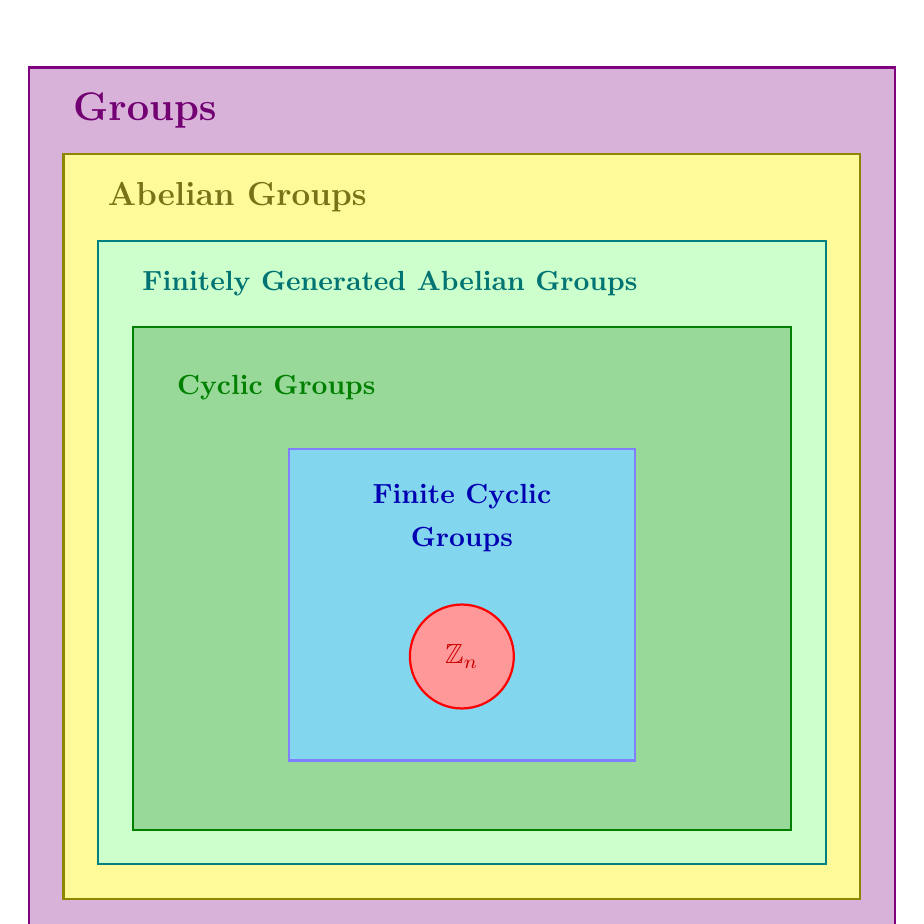
\begin{tikzpicture}[scale=1.1, font=\sffamily]
			
			% Groups
			\draw[fill=violet!30, draw=violet, thick] (0,0) rectangle (10,10);
			\node[text=violet!90!black, font=\bfseries\Large, anchor=west] at (0.4, 9.5) {Groups};
			
			% Abelian Groups
			\draw[fill=yellow!40, draw=olive, thick] (0.4, 0.4) rectangle (9.6, 9.0);
			\node[text=olive!80!black, font=\bfseries\large, anchor=west] at (0.8, 8.5) {Abelian Groups};
			
			% Finitely Generated Abelian Groups
			\draw[fill=green!20, draw=teal, thick] (0.8, 0.8) rectangle (9.2, 8.0);
			\node[text=teal!90!black, font=\bfseries, anchor=west] at (1.2, 7.5) {Finitely Generated Abelian Groups};
			
			% Cyclic Groups
			\draw[fill=green!40!black, fill opacity=0.25, draw=green!50!black, thick] (1.2, 1.2) rectangle (8.8, 7.0);
			\node[text=green!50!black, font=\bfseries, anchor=west, opacity=1] at (1.6, 6.3) {Cyclic Groups};
			
			% Finite Cyclic Groups
			\draw[fill=cyan!50, draw=blue!50, thick, fill opacity=0.9] (3.0, 2.0) rectangle (7.0, 5.6);
			\node[text=blue!70!black, font=\bfseries, align=center] at (5.0, 4.8) {Finite Cyclic\\[0.3em]Groups};
			
			% Z_n 
			\draw[fill=red!40, draw=red, thick, fill opacity=1] (5.0, 3.2) circle (0.6);
			\node[text=red!80!black, font=\bfseries] at (5.0, 3.2) {$\Z_n$};
			
		\end{tikzpicture}
		\vfill
		
		% Author and Lecturer Details
		\vspace{1cm}
		\begin{minipage}{0.45\textwidth}
			\begin{flushleft}
				\textit{Written by:}\\
				\textbf{Mohamed Asubhi}
			\end{flushleft}
		\end{minipage}
		\begin{minipage}{0.45\textwidth}
			\begin{flushright}
				\textit{Lecturer:}\\
				\textbf{Prof. Mohamed Ramadan}
			\end{flushright}
		\end{minipage}\\[2.5em]
		
		% Date / Term
		{\large Fall Term 2026}
	\end{titlepage}
	
	\newpage
	
	% ==========================================
	% FRONT MATTER (ROMAN NUMERALS)
	% ==========================================
	\pagenumbering{roman} 
	\pagestyle{plain} 
	
	% ==========================================
	% TABLE OF CONTENTS
	% ==========================================
	\vspace*{1em}
	\noindent\rule{\textwidth}{1.2pt} \\[-0.85\baselineskip]
	\noindent\rule{\textwidth}{0.4pt}
	\begin{center}
		\huge \textsc{Contents}
	\end{center}
	\vspace{1.5em}
	
	\tableofcontents
	
	\newpage
	% ==========================================
	% ACKNOWLEDGMENTS (LARGER TEXT)
	% ==========================================
	\vspace*{1em}
	\noindent\rule{\textwidth}{1.2pt} \\[-0.85\baselineskip]
	\noindent\rule{\textwidth}{0.4pt}
	\begin{center}
		\huge \textsc{Acknowledgments}
	\end{center}
	\vspace{2em}
	
	{
		
		First and foremost, I would like to express my sincere gratitude to \textbf{Prof. Mohamed Ramadan}. These notes are based on his lectures, and I am deeply thankful for the foundational material he provided and his dedicated work with us.
		
		\vspace{1.5em}
		Special thanks to my friend \textbf{Mina Basilious} who helped very much in refining the text, and checked most of the proofs and material.
	}
	
	
	
	
	\newpage
	% ==========================================
	% MAIN CONTENT (ARABIC NUMERALS & FANCY HEADERS)
	% ==========================================
	\pagenumbering{arabic}
	\pagestyle{fancy}
	\fancyhf{}
	\lhead{\textbf{M311: Abstract Algebra}}
	% \rhead{\leftmark}
	% \lfoot{\textit{Dept. of Math, Cairo University}}
	\cfoot{\thepage}
	
	\lecturetitle{1}{Introduction to Groups \& Fundamental Algebraic Structures}
	\rhead{Lecture 1: Fundamental Structures}
	% \textit{Date: Sep 23, 2026}
	
	\subsection{Congruence Modulo $n$}
	
	\begin{definition}{Congruence Modulo $n$}
		Let $a, b \in \Z$ and $n \in \Z^+$. We say that $a$ is congruent to $b$ modulo $n$ if $n$ divides $(a - b)$. We denote it by:
		\[
		a \equiv b \pmod{n} \quad \text{or} \quad a \equiv_n b
		\]
		Equivalently:
		\[
		a \equiv b \pmod{n} \iff n \mid (a - b) \iff \exists k \in \Z, \; a - b = n k \iff \exists k \in \Z, \; a = b + n k.
		\]
	\end{definition}
	
	\begin{example}
		\begin{itemize}
			\item $17 \equiv 5 \pmod{6}$ and $5 \equiv 17 \pmod{6}$.
			\item $17 \equiv 17 \pmod{n}$ for all $n \in \Z^+$.
			\item $2 \equiv -4 \pmod{6}$ and $-4 \equiv 8 \pmod{6} \implies 2 \equiv 8 \pmod{6}$.
		\end{itemize}
	\end{example}
	
	\begin{proposition}[Congruence is an Equivalence]
		The relation $\equiv_n$ is reflexive, symmetric, and transitive. Hence, $\equiv_n$ is an equivalence relation on $\Z$, \textcolor{red}{(Ex: Prove it)}.
	\end{proposition}
	
	\begin{definition}{Equivalence Class}
		The relation $\equiv_n$ partitions $\Z$ into $n$ equivalence classes. The equivalence class generated by $a \in \Z$ is denoted $\bar{a}$ or $[a]$ and is defined as:
		\[
		\bar{a} = \{ b \in \Z \mid b \equiv a \pmod{n} \} = \{ b \in \Z \mid b = a + nk, \; k \in \Z \} = \{ a + nk \mid k \in \Z \}
		\]
	\end{definition}
	
	\begin{example}[Equivalence Classes for $n = 3$]
		\begin{itemize}
			\item $\bar{0} = \{ 0 + 3k \mid k \in \Z \} = \{ \dots, -6, -3, 0, 3, 6, \dots \}$
			\item $\bar{1} = \{ 1 + 3k \mid k \in \Z \} = \{ \dots, -5, -2, 1, 4, 7, \dots \}$
			\item $\bar{2} = \{ 2 + 3k \mid k \in \Z \} = \{ \dots, -4, -1, 2, 5, 8, \dots \}$
		\end{itemize}
	\end{example}
	
	\begin{definition}{The Set $\Z_n$}
		We denote the set of equivalence classes modulo $n$ as:
		\[
		\Z_n = \{ \bar{0}, \bar{1}, \bar{2}, \dots, \overline{n-1} \}
		\]
		We define binary operations $\oplus$ and $\otimes$ on $\Z_n$ by:
		\[
		\forall \bar{a}, \bar{b} \in \Z_n, \quad \bar{a} \oplus \bar{b} = \overline{a + b} \quad \text{and} \quad \bar{a} \otimes \bar{b} = \overline{a \cdot b}
		\]
		One checks that $\oplus, \otimes$ are well-defined binary operations on $\Z_n$ (the result does not depend on the chosen representatives).
	\end{definition}
	
	\begin{proposition}[Group Structures on $\Z_n$]
		$(\Z_n, \oplus)$ is an abelian group for any $n \ge 1$. However, for $n \ge 2$, $(\Z_n, \otimes)$ is not a group because $\bar{0}$ has no multiplicative inverse.
	\end{proposition}
	
	\begin{example}
		The Cayley tables for $(\Z_5, \oplus)$ and $(\Z_5, \otimes)$ are presented below:
		
		\begin{center}
			\begin{minipage}{0.48\textwidth}
				\centering
				\textbf{Addition Modulo 5 ($\oplus$)} \\[0.5em]
				\[
				\begin{array}{c|ccccc}
					\oplus & \bar{0} & \bar{1} & \bar{2} & \bar{3} & \bar{4} \\ \hline
					\bar{0} & \bar{0} & \bar{1} & \bar{2} & \bar{3} & \bar{4} \\
					\bar{1} & \bar{1} & \bar{2} & \bar{3} & \bar{4} & \bar{0} \\
					\bar{2} & \bar{2} & \bar{3} & \bar{4} & \bar{0} & \bar{1} \\
					\bar{3} & \bar{3} & \bar{4} & \bar{0} & \bar{1} & \bar{2} \\
					\bar{4} & \bar{4} & \bar{0} & \bar{1} & \bar{2} & \bar{3}
				\end{array}
				\]
			\end{minipage}
			\hfill
			\begin{minipage}{0.48\textwidth}
				\centering
				\textbf{Multiplication Modulo 5 ($\otimes$)} \\[0.5em]
				\[
				\begin{array}{c|ccccc}
					\otimes & \bar{0} & \bar{1} & \bar{2} & \bar{3} & \bar{4} \\ \hline
					\bar{0} & \bar{0} & \bar{0} & \bar{0} & \bar{0} & \bar{0} \\
					\bar{1} & \bar{0} & \bar{1} & \bar{2} & \bar{3} & \bar{4} \\
					\bar{2} & \bar{0} & \bar{2} & \bar{4} & \bar{1} & \bar{3} \\
					\bar{3} & \bar{0} & \bar{3} & \bar{1} & \bar{4} & \bar{2} \\
					\bar{4} & \bar{0} & \bar{4} & \bar{3} & \bar{2} & \bar{1}
				\end{array}
				\]
			\end{minipage}
		\end{center}
		\textbf{Why $(\Z_5, \oplus)$ is an Abelian Group:}
		\begin{enumerate}[leftmargin=2em]
			\item \textbf{Closure:} Every entry in the addition table belongs to $\Z_5$.
			\item \textbf{Associativity:} Inherited from the associativity of integer addition.
			\item \textbf{Identity Element:} $\bar{0}$ acts as the additive identity ($\bar{a} \oplus \bar{0} = \bar{a}$).
			\item \textbf{Inverse Elements:} Every element has an additive inverse: 
			$\bar{0}^{-1} = \bar{0}$, $\bar{1}^{-1} = \bar{4}$, $\bar{2}^{-1} = \bar{3}$, $\bar{3}^{-1} = \bar{2}$, and $\bar{4}^{-1} = \bar{1}$.
			\item \textbf{Commutativity:} The addition table is symmetric along its main diagonal, meaning $\bar{a} \oplus \bar{b} = \bar{b} \oplus \bar{a}$.
		\end{enumerate}
		\textbf{Why $(\Z_5, \otimes)$ is NOT a Group:}
		Although multiplication is associative, commutative, and has an identity element ($\bar{1}$), \textbf{it fails the inverse axiom}. 
		Specifically, the element $\bar{0}$ has no multiplicative inverse because there is no element $x \in \Z_5$ such that $\bar{0} \otimes x = \bar{1}$.
		
	\end{example}
	
	\begin{remark}
		If $p$ is a prime number, then $\Z_p^* = \Z_p \setminus \{ \bar{0} \}$ forms an abelian group under multiplication $(\Z_p^*, \otimes)$.
	\end{remark}
	
	% ------------------------------------------
	
	\subsection{Groups, Order of Group, and Order of Elements}
	
	\begin{definition}{Order of a Group}
		Let $G$ be a group. The \textbf{order} of $G$, denoted $|G|$, is the number of distinct elements in $G$.
		\begin{itemize}
			\item If $|G|$ is finite, $G$ is called a \textbf{finite group}.
			\item If $|G|$ is infinite, $G$ is called an \textbf{infinite group}.
		\end{itemize}
	\end{definition}
	
	\begin{example}[Group Orders]
		\begin{itemize}
			\item $(\Z, +)$ is an infinite group since $|\Z|$ is infinite.
			\item $G = \{1, -1, i, -i\}$ under complex multiplication is a finite group of order $|G| = 4$.
		\end{itemize}
	\end{example}
	
	\begin{definition}{Order of an Element}
		Let $G$ be a group and $a \in G$. The \textbf{order of $a$}, denoted $|a|$, is the least positive integer $n$ such that:
		\[
		a^n = e
		\]
		where $e$ is the identity element of $G$. If no such positive integer exists, we say $a$ has infinite order.
	\end{definition}
	
	\begin{example}[Computing Element Orders]
		\textbf{a)} In $G = \{1, -1, i, -i\}$ with $e = 1$:
		\begin{itemize}
			\item $(1)^1 = 1 \implies |1| = 1$
			\item $(-1)^1 = -1, \; (-1)^2 = 1 \implies |-1| = 2$
			\item $(i)^1 = i, \; (i)^2 = -1, \; (i)^3 = -i, \; (i)^4 = 1 \implies |i| = 4$ and $|{-i}| = 4$
		\end{itemize}
		
		\textbf{b)} In $(\Z_6, \oplus)$ with identity element $e = \bar{0}$:
		\begin{itemize}
			\item $1\cdot\bar{0} = \bar{0} \implies |\bar{0}| = 1$
            \item $1\cdot\bar{1} = \bar{1}, \; 2\cdot\bar{1} = \bar{2}, \; 3\cdot\bar{1} = \bar{3}, \; 4\cdot\bar{1} = \bar{4}, \; 5\cdot\bar{1} = \bar{5}, \; 6\cdot\bar{1} = \bar{0} \implies |\bar{1}| = 6$
            \item $1\cdot\bar{2} = \bar{2}, \; 2\cdot\bar{2} = \bar{4}, \; 3\cdot\bar{2} = \bar{0} \implies |\bar{2}| = 3$
		\end{itemize}
	\end{example}
	
	% ------------------------------------------
	
	\subsection{Cyclic Groups}
	\begin{definition}{Generator of a Group}
		Let $G$ be a group and $a \in G$. The \textbf{cyclic subgroup generated by $a$} is the set:
		\[
		\langle a \rangle = \{ a^n \mid n \in \Z \}
		\]
		
	\end{definition}
	\begin{definition}{Cyclic Group}
		A group $G$ is called \textbf{cyclic} if there exists an element $a \in G$ such that:
		\[
		G = \langle a \rangle
		\]
	\end{definition}
	\begin{proposition}[Properties of Cyclic Groups]
		Let $G = \langle a \rangle$ be a cyclic group.
		\begin{enumerate}
			\item $G = \langle a \rangle \iff G = \langle a^{-1} \rangle$.
			\item $|G| = |\langle a \rangle| = |a|$.
			\item Every cyclic group is abelian.
		\end{enumerate}
	\end{proposition}
	
	\begin{example}[Examples of Cyclic Groups]
		\begin{itemize}
			\item $(\Z_n, \oplus) = \langle \bar{1} \rangle$ is a finite cyclic group of order $n$.
			\item $(\Z, +) = \langle 1 \rangle = \langle -1 \rangle$ is an infinite cyclic group.
		\end{itemize}
	\end{example}
	
	\begin{theorem}[Subgroups of $\Z$]
		Every subgroup of $(\Z, +)$ is cyclic and is of the form $n\Z = \langle n \rangle$ for some $n \in \Z^{\ge 0}$.
	\end{theorem}
	
	% ------------------------------------------
	
	\subsection{Permutation Groups and Symmetric Groups}
	
	\noindent\textit{Convention: permutations are composed from right to left.}
	
	\begin{definition}{Permutation}
		Let $X$ be a non-empty set. A \textbf{permutation} of $X$ is a function $f: X \to X$ that is both one-to-one (injective) and onto (surjective), i.e., a bijective function.
	\end{definition}
	
	\begin{notation}{Function as an Array}
		Let $X = \{x_1, x_2, \ldots, x_n\}$ be a finite set. Then we write a function $f : X \to X$ as an array
		\[
			f = \begin{pmatrix}
				x_1 & x_2 & \cdots & x_n \\
				f(x_1) & f(x_2) & \cdots & f(x_n)
			\end{pmatrix},
		\]
		where the first row lists the inputs and the second row lists the corresponding outputs.
	\end{notation}

	\begin{example}
		Let $X=\{1,2\}$ and construct every possible function on the set, we get 4 functions: 
		\[
		f_1 = \begin{pmatrix} 1 & 2  \\ 1 & 2  \end{pmatrix}, \quad 
		f_2 = \begin{pmatrix} 1 & 2  \\ 2 & 1  \end{pmatrix}, \quad 
		f_3 = \begin{pmatrix} 1 & 2  \\ 1 & 1  \end{pmatrix}, \quad
		f_4 = \begin{pmatrix} 1 & 2  \\ 2 & 2  \end{pmatrix}.
		\]
		But $f_1, f_2$ are the only permutations on $X$; we denote them by $\sigma_1, \sigma_2$
		\[
		\sigma_1 = \begin{pmatrix} 1 & 2  \\ 1 & 2  \end{pmatrix} =(1), \quad 
		\sigma_2 = \begin{pmatrix} 1 & 2  \\ 2 & 1  \end{pmatrix}= (12).
		\]
	\end{example}
	
	\begin{definition}{Symmetric Group $S_n$}
		The set of all permutations on a set of $n$ elements $X_n = \{1, 2, \dots, n\}$ under function composition $\circ$ forms a group called the \textbf{Symmetric Group on $n$ letters}, denoted $S_n$.
		The order of $S_n$ is:
		\[
		|S_n| = n!
		\]
	\end{definition}
	
	\begin{example}
		For $X = \{1, 2, 3\}$. We get 27 functions but 6 only are bijective:
		\[
		S_3 = \{ \sigma_1, \sigma_2, \sigma_3, \sigma_4, \sigma_5, \sigma_6 \}
		\]
		where:
		\[
		\sigma_1 = \begin{pmatrix} 1 & 2 & 3 \\ 1 & 2 & 3 \end{pmatrix}, \quad 
		\sigma_2 = \begin{pmatrix} 1 & 2 & 3 \\ 2 & 1 & 3 \end{pmatrix}, \quad 
		\sigma_3 = \begin{pmatrix} 1 & 2 & 3 \\ 1 & 3 & 2 \end{pmatrix}
		\]
		\[
		\sigma_4 = \begin{pmatrix} 1 & 2 & 3 \\ 3 & 2 & 1 \end{pmatrix}, \quad 
		\sigma_5 = \begin{pmatrix} 1 & 2 & 3 \\ 2 & 3 & 1 \end{pmatrix}, \quad 
		\sigma_6 = \begin{pmatrix} 1 & 2 & 3 \\ 3 & 1 & 2 \end{pmatrix}
		\]
	\end{example}
	
	\begin{definition}{Cycle and Transposition}
	A \textbf{cycle} $(a_1\, a_2\, \dots\, a_k)$ is the permutation sending $a_1 \mapsto a_2 \mapsto \dots \mapsto a_k \mapsto a_1$ and fixing all other elements.
	A cycle of length $2$ is called a \textbf{transposition}.
\end{definition}

\begin{proposition}
	Every permutation $\sigma \in S_n$ is a product of transpositions, e.g.
	\[
	(a_1 a_2 a_3 \dots a_k) = (a_1 a_k)(a_1 a_{k-1})\dots(a_1 a_2).
	\]
	The parity (even or odd) of the number of transpositions is the same for every such expression of $\sigma$.
\end{proposition}

\begin{definition}{Even and Odd Permutations}
	\begin{itemize}
		\item If $\sigma$ is a product of an \textbf{even} number of transpositions, $\sigma$ is an \textbf{even permutation}.
		\item If $\sigma$ is a product of an \textbf{odd} number of transpositions, $\sigma$ is an \textbf{odd permutation}.
	\end{itemize}
\end{definition}
	
	\begin{definition}{Alternating Group $A_n$}
		The group of all \textbf{even permutations} in $S_n$ is called the \textbf{Alternating Group} of degree $n$, denoted $A_n$. For $n \ge 2$, its order is:
		\[
		|A_n| = \frac{n!}{2}
		\]
	\end{definition}
	
	\begin{caution}
		Permutation composition is generally non-commutative ($S_n$ is non-abelian for $n \ge 3$). In these notes, composition is evaluated right-to-left.
	\end{caution}
	
	% ------------------------------------------
	
	\subsection{Cartesian Product of Sets and Groups}
	
	\begin{definition}{Cartesian Product}
		Let $A$ and $B$ be non-empty sets. The \textbf{Cartesian Product} $A \times B$ is defined by:
		\[
		A \times B = \{ (a, b) \mid a \in A, \, b \in B \}
		\]
		If $A$ and $B$ are finite with $|A| = n$ and $|B| = m$, then $|A \times B| = n \cdot m$.
	\end{definition}
	
	\begin{example}
		\begin{itemize}
			\item Let $A = \{2, 3\}$ and $B = \{1, 2, 4\}$. Then:
			\[
			A \times B = \{ (2,1), (2,2), (2,4), (3,1), (3,2), (3,4) \}
			\]
			\item 
			\(
			\R \times \R =\{(x,y) \mid x,y \in \R\} = \R^2 
			\) 
			\item 
			\(
			\R^n = \underbrace{\mathbb{R} \times \mathbb{R} \times \cdots \times \mathbb{R}}_{n \text{ times}} =\{(a_1,a_2,\dots,a_n) \mid a_i \in \R\} 
			\) 
		\end{itemize}
	\end{example}
	
	\begin{notation}{Iterated Product}
		For a set $A$, we write $A^n$ to mean the $n$-fold Cartesian product, defined recursively on $n$; equivalently,
		\[
			A^n = \underbrace{A \times A \times \cdots \times A}_{n\text{ times}}.
		\]
	\end{notation}
	
	\lecturetitle{2}{External Direct Product}
	% \textit{Date: Sep 28, 2026}
	
	\subsection{External Direct Product}
	
	\begin{definition}{External Direct Product}
		Let $(H, \cdot)$ and $(K, \circ)$ be groups.
		The Cartesian product $H \times K$ can be made into a group by defining a binary operation $*$ on $H \times K$ as follows:
		\[
		(a_1, b_1) * (a_2, b_2) := (a_1 \cdot a_2, b_1 \circ b_2) \in H \times K
		\]
		This forms a group called the \textbf{external direct product}.
	\end{definition}
	
	\begin{theorem}
		The set $H \times K$ with the operation $*$ forms a group.
	\end{theorem}
	\begin{proof}
		We verify the group axioms for $H \times K$:
		\begin{enumerate}
			\item \textbf{Closure:} The operation $*$ is a binary operation on $H \times K$.
			\item \textbf{Associativity:} For any $(a_1, b_1), (a_2, b_2), (a_3, b_3) \in H \times K$:
			\begin{align*}
				((a_1, b_1) * (a_2, b_2)) * (a_3, b_3) &= (a_1 \cdot a_2, b_1 \circ b_2) * (a_3, b_3) \\
				&= ((a_1 \cdot a_2) \cdot a_3, (b_1 \circ b_2) \circ b_3) \\
				&= (a_1 \cdot (a_2 \cdot a_3), b_1 \circ (b_2 \circ b_3)) \\
				&= (a_1, b_1) * (a_2 \cdot a_3, b_2 \circ b_3) \\
				&= (a_1, b_1) * ((a_2, b_2) * (a_3, b_3))
			\end{align*}
			Thus, $*$ is associative.
			
			\item \textbf{Identity:} $(e_H, e_K)$ works, since $(a,b)*(e_H,e_K) = (a,b) = (e_H,e_K)*(a,b)$.
			
			\item \textbf{Inverse:} For any $(a, b) \in H \times K$, the inverse is $(a, b)^{-1} = (a^{-1}, b^{-1})$. 
			Indeed:
			\[
			(a, b) * (a^{-1}, b^{-1}) = (e_H, e_K) = (a^{-1}, b^{-1}) * (a, b).
			\]
		\end{enumerate}
	\end{proof}
	
	\begin{remark}
		\begin{itemize}
			\item Neither $H$ nor $K$ are subgroups of $H \times K$.
			\item However, subsets of the form $H \times \{e_K\}$ and $\{e_H\} \times K$ are subgroups of $H \times K$, \textcolor{red}{(Ex: Prove it)}.
			\item Moreover, $H \times \{e_K\} \cong H$ and $\{e_H\} \times K \cong K$, \textcolor{red}{(Ex: Prove it)}.
		\end{itemize}
	\end{remark}
	
	\begin{recall}
		Let $H \leq G$, we say that $H \trianglelefteq G$ if and only if one of the following equivalent conditions holds:
		\begin{enumerate}
			\item $Ha = aH, \quad \forall a \in G$
			\item $a^{-1}Ha = H, \quad \forall a \in G$,
			\item $aHa^{-1} = H, \quad \forall a \in G$,
			\item $aha^{-1} \in H, \quad \forall a \in G,\ h \in H$.
		\end{enumerate}
		Moreover, if $G$ is abelian, $H\leq G \implies H \trianglelefteq G$. \textcolor{red}{(Ex: Prove it)}
	\end{recall}
	
	\begin{remark}
		In general, if $G_1, G_2, \dots, G_n$ are groups, we define an operation on the Cartesian product $G_1 \times \dots \times G_n$ component-wise:
		\[
		(a_1, \dots, a_n) * (b_1, \dots, b_n) = (a_1 \cdot_1 b_1, \dots, a_n \cdot_n b_n)
		\]
		Thus, $(G_1 \times \dots \times G_n, *)$ is called the external direct product of $G_1, \dots, G_n$. We denote it by $\prod_{i=1}^{n} G_i$ or $G_1 \otimes \cdots \otimes G_n$. If the operation on each $G_i$ is addition, we write $\bigoplus_{i=1}^n G_i$ instead of $\prod_{i=1}^{n} G_i$ and call it the \textbf{external direct sum} of $G_1, G_2, \dots, G_n$.\footnote{In full generality, the external direct sum is defined for arbitrary families of groups; this is beyond the scope of this course. For finitely many groups, however, it is equivalent to the direct product.}
	\end{remark}
	
	
	\subsection{Properties of the Direct Product}
	
	\begin{theorem}
		Let $G_1, G_2$ be groups. Then $G_1 \times G_2$ is abelian if and only if $G_1, G_2$ are abelian.
	\end{theorem}
	
	\begin{proof}
		($\Rightarrow$) Suppose $G_1 \times G_2$ is abelian.
		Let $(a_1, b_1), (a_2, b_2) \in G_1 \times G_2$, where $a_1, a_2 \in G_1$ and $b_1, b_2 \in G_2$. 
		Because the group is abelian:
		\[
		(a_1, b_1)(a_2, b_2) = (a_2, b_2)(a_1, b_1)
		\]
		This implies $(a_1 a_2, b_1 b_2) = (a_2 a_1, b_2 b_1)$.
		Therefore, $a_1 a_2 = a_2 a_1$ and $b_1 b_2 = b_2 b_1$. 
		Hence, both $G_1$ and $G_2$ are abelian.
		
		\vspace{0.5em}
		\noindent ($\Leftarrow$) Suppose $G_1$ and $G_2$ are abelian. 
		For any $(a_1, b_1), (a_2, b_2) \in G_1 \times G_2$:
		\[
		(a_1, b_1)(a_2, b_2) = (a_1 a_2, b_1 b_2)
		\]
		Since $G_1$ and $G_2$ are abelian, $a_1 a_2 = a_2 a_1$ and $b_1 b_2 = b_2 b_1$.
		Thus:
		\[
		(a_1 a_2, b_1 b_2) = (a_2 a_1, b_2 b_1) = (a_2, b_2)(a_1, b_1)
		\]
		Therefore, $G_1 \times G_2$ is abelian.
	\end{proof}
	
	\begin{caution}
		If $G_1, G_2$ are cyclic, $G_1 \times G_2$ is not necessarily cyclic.
	\end{caution}
	
	\subsection{Examples of Direct Products}
	
	\begin{example}
		Consider $G = \Z \times \Z = \{(x, y) \mid x, y \in \Z\}$. 
		While it is abelian, $\Z \times \Z$ is not cyclic. 
		Suppose $\Z \times \Z = \langle(x,y)\rangle$. Then $(1,0) = k(x,y)$ and $(0,1) = m(x,y)$ for some $k, m \in \Z$.
		Since $kx = 1$ we have $k \neq 0$ and $x = \pm 1$; then $ky = 0$ gives $y = 0$. But then $my = 0 \neq 1$, a contradiction.
		Hence $\Z \times \Z$ is not cyclic.
	\end{example}
	
	\begin{example}
		Let $G_1 = (\Z_4, \oplus)$ and $G_2 = (S_3, \circ)$. 
		We have:
		\[
		G_1 = \{\bar{0}, \bar{1}, \bar{2}, \bar{3}\}
		\]
		\[
		G_2 = \{(1), (12), (13), (23), (123), (132)\}
		\]
		It is known that $G_1$ is abelian, but $G_2$ is not abelian. 
		Let us check if $G_1 \times G_2$ is abelian by taking two elements $(\bar{3}, (123))$ and $(\bar{2}, (13))$:
		\begin{align*}
			(\bar{3}, (123)) * (\bar{2}, (13)) &= (\bar{3} \oplus \bar{2}, (123)(13)) = (\bar{1}, (23)) \\
			(\bar{2}, (13)) * (\bar{3}, (123)) &= (\bar{2} \oplus \bar{3}, (13)(123)) = (\bar{1}, (12))
		\end{align*}
		Since $(\bar{1}, (23)) \neq (\bar{1}, (12))$, the product $G_1 \times G_2$ is not abelian.
	\end{example}
	
	\begin{example}
		Consider $\Z_2 \times \Z_2 = \{(\bar{0},\bar{0}), (\bar{0},\bar{1}), (\bar{1},\bar{0}), (\bar{1},\bar{1})\}$. 
		The group $\Z_2 \times \Z_2$ is abelian but not cyclic, since every non-identity element has order $2 < 4$.
	\end{example}
	
	\begin{example}
		Consider $\Z_2 \times \Z_3$. 
		\[ \Z_2 = \{\bar{0}, \bar{1}\}, \quad \Z_3 = \{\bar{0}, \bar{1}, \bar{2}\} \] 
		Let us compute the powers (multiples) of the element $(\bar{1}, \bar{1})$:
		\begin{align*}
			1 \cdot (\bar{1}, \bar{1}) &= (\bar{1}, \bar{1}) \\
			2 \cdot (\bar{1}, \bar{1}) &= (\bar{0}, \bar{2}) \\
			3 \cdot (\bar{1}, \bar{1}) &= (\bar{1}, \bar{0}) \\
			4 \cdot (\bar{1}, \bar{1}) &= (\bar{0}, \bar{1}) \\
			5 \cdot (\bar{1}, \bar{1}) &= (\bar{1}, \bar{2}) \\
			6 \cdot (\bar{1}, \bar{1}) &= (\bar{0}, \bar{0})
		\end{align*}
		Since $|(\bar{1}, \bar{1})| = 6$, we see that $\Z_2 \times \Z_3 = \langle(\bar{1}, \bar{1})\rangle$. 
		Thus, it is cyclic.
	\end{example}
	
	\begin{example}
		Consider $\Z_2 \times \Z_4 = \{(\bar{0},\bar{0}), (\bar{0},\bar{1}), (\bar{0},\bar{2}), (\bar{0},\bar{3}), (\bar{1},\bar{0}), (\bar{1},\bar{1}), (\bar{1},\bar{2}), (\bar{1},\bar{3})\}$.
		This group is not cyclic because it does not contain an element of order $8$. 
	\end{example}
	
	\subsection{Cyclic Isomorphisms in Direct Products}

    \begin{recall}
		This property is not specific to $\Z_n$. In fact, for any cyclic group $G = \langle a \rangle$:
		\begin{itemize}[leftmargin=2em]
			\item If $|a| = n$ (finite order), then $G \cong \Z_n$.
			\item If $|a| = \infty$ (infinite order), then $G \cong \Z$.
		\end{itemize}
	\end{recall}
    
	\begin{theorem}
		The group $\Z_n \times \Z_m$ is cyclic if and only if $\gcd(n,m) = 1$. In that case, $\Z_n \times \Z_m \cong \Z_{nm}$.
	\end{theorem}
	
	\begin{proof}
		We prove both directions of the equivalence explicitly:
		
		\vspace{0.5em}
		\noindent \textbf{($\Rightarrow$)} Suppose that $\Z_n \times \Z_m$ is cyclic.
		
		Assume for the sake of contradiction that $\gcd(n,m) \neq 1$. Let $d = \gcd(n,m) > 1$, which means $d$ divides both $n$ and $m$ ($d|n$ and $d|m$). Let $(a, b)$ be any arbitrary element in $\Z_n \times \Z_m$. 
		
		Consider the multiple $\frac{nm}{d}$ of $(a, b)$:
		\[
		\frac{nm}{d} (a, b) = \left( a \frac{nm}{d}, b \frac{nm}{d} \right) = \left( \frac{m}{d}(na), \frac{n}{d}(mb) \right) = (\bar{0}, \bar{0})
		\]
		This demonstrates that the order $|(a, b)| \leq \frac{nm}{d} < nm$. Consequently, every single element in $\Z_n \times \Z_m$ has an order strictly less than the order of the group itself ($|\Z_n \times \Z_m| = nm$). Because no element can generate a group of size $nm$, $\Z_n \times \Z_m$ cannot be cyclic, which contradicts our initial assumption. Therefore, we must have $\gcd(n,m) = 1$.
		
		\vspace{0.8em}
		\noindent \textbf{($\Leftarrow$)} Suppose now that $\gcd(n,m) = 1$. 
		
		We know that $\Z_n = \langle\bar{1}\rangle$ and $\Z_m = \langle\bar{1}\rangle$. Consider the element $(\bar{1}, \bar{1}) \in \Z_n \times \Z_m$ and let $H = \langle(\bar{1}, \bar{1})\rangle$ be the cyclic subgroup it generates. 
		
		In $\Z_n$ we have $n\cdot\bar{1} = \bar{0}$, hence $nm\cdot\bar{1} = \bar{0}$; similarly $m\cdot\bar{1} = \bar{0}$ in $\Z_m$, hence $nm\cdot\bar{1} = \bar{0}$. 
		Raising $(\bar{1}, \bar{1})$ to the power $nm$ yields:
		\[
		nm\cdot(\bar{1}, \bar{1}) = (nm\cdot\bar{1}, nm\cdot\bar{1}) = (\bar{0}, \bar{0})
		\]
		This establishes that the order satisfies $|(\bar{1}, \bar{1})| \leq nm$.
		
		Now, assume there exists some positive integer $s < nm$ such that $|(\bar{1}, \bar{1})| = s$. Then $s\cdot(\bar{1}, \bar{1}) = (\bar{0}, \bar{0})$, meaning $(s\cdot\bar{1}, s\cdot\bar{1}) = (\bar{0}, \bar{0})$. This implies that $n|s$ and $m|s$. Because $\gcd(n,m) = 1$, their least common multiple $nm$ must divide $s$ ($nm | s$). Thus, $s$ cannot be strictly less than $nm$, forcing $s = nm$. 
		
		Therefore, $|(\bar{1}, \bar{1})| = nm$, which means the subgroup size is $|H| = nm = |\Z_n \times \Z_m|$. This proves that $\Z_n \times \Z_m = \langle(\bar{1}, \bar{1})\rangle$, making the group cyclic. Since it is cyclic of order $nm$, it is isomorphic to $\Z_{nm}$.
	\end{proof}
	
	
	
	\begin{proposition}
		Let $G$ and $H$ be finite cyclic groups. 
		\[
		G \times H \text{ is cyclic } \iff \gcd(|G|, |H|) = 1.
		\] 
	\end{proposition}
	
\begin{exercise}
	\subsection*{Problem Set 1}
	\begin{enumerate}
		\item Let $H$ and $K$ be finite cyclic groups. Prove that $H \times K \text{ is cyclic } \iff \gcd(|H|, |K|) = 1$.
		
		\item Let $G$ be a cyclic group. Then:
		\begin{enumerate}[label=(\roman*)]
			\item If $G$ is finite of order $n$, prove that $G \cong \Z_n$.
			\item If $G$ is infinite, prove that $G \cong \Z$.
		\end{enumerate}
		
		\item Let $G$ be a group with identity $e$. If $x^2 = e$ for every $x \in G$, show that $G$ is abelian. \label{ex:square-abelian}
	\end{enumerate}
	
	\subsection*{Problem Set 2}
	\begin{enumerate}
		\item If $(H, \cdot)$ and $(K, \circ)$ are groups, verify that $H \times \{e_K\}$ and $\{e_H\} \times K$ are normal subgroups of $H \times K$.
		
		\item Let $G = \langle a, b \mid a^4 = b^2 = e,\ ab = ba^3 \rangle$, and set $H = \langle a \rangle$ and $K = \langle b \rangle$. Is $H \trianglelefteq G$? Is $K \trianglelefteq G$? Explain your answer.
		
		\item Suppose that $A = \langle(1234)\rangle$ and $B = A_4$, verify that $|A \cap B| = 2$. Does $S_4 = AB$? Explain your answer.
		
		\item Let $A \le G$ and $B \le G$, where $G$ is a finite group. Show that:
		\[
		|AB| = \frac{|A||B|}{|A \cap B|}
		\]
		
		\item Let $A = S_3$ (viewed as the subgroup of $S_4$ fixing $4$) and $B = \{(1), (12), (34), (12)(34)\}$. Prove that $AB$ is not a subgroup of $S_4$.
		
		\item If $C = \langle(123)\rangle$ and $K = \{(1), (12)(34), (13)(24), (14)(23)\}$, verify that $A_4 = KC$.
		
		\item If $G_1$ and $G_2$ are cyclic groups of order $m$ and $n$, respectively, prove that $G_1 \times G_2$ is cyclic if and only if $m$ and $n$ are relatively prime.
	\end{enumerate}
\end{exercise}

	\lecturetitle{3}{Internal Direct Product}
	% \textit{Date: Sep 30, 2026}
	
	
	\begin{corollary}
		Let $p_1, \dots, p_n$ be primes and $e_i \ge 1$. Then
		\[
		\Z_{p_1^{e_1}} \times \dots \times \Z_{p_n^{e_n}} \cong \Z_{p_1^{e_1} \cdots p_n^{e_n}} \iff p_i \neq p_j, \quad \forall\, i \neq j.
		\]
	\end{corollary}
	
	
	\begin{example}
		\begin{itemize}
			\item $\Z_8 \times \Z_9 = \Z_{2^3} \times \Z_{3^2} \cong \Z_{72}$, since $\gcd(8, 9) = 1$.
			\item Is $\Z_2 \times \Z_5 \times \Z_4 \cong \Z_{40}$? Why?
		\end{itemize}
		\vspace{0.5em}
		\noindent \textbf{Solution:}
		\begin{align*}
			\Z_2 \times \Z_5 \times \Z_4 &\cong \Z_{10} \times \Z_4, \quad \gcd(2,5)=1.
		\end{align*}
		Since $\gcd(10,4) = 2 \neq 1$, the group $\Z_{10} \times \Z_4$ is not cyclic, whereas $\Z_{40}$ is cyclic. Hence $\Z_2 \times \Z_5 \times \Z_4 \ncong \Z_{40}$, and the answer is \textbf{no}.
	\end{example}
		
\begin{example}
    Show that every group of order $4$ is isomorphic to $\Z_4$ or to $\Z_2 \times \Z_2$.
\end{example}

\begin{proof}
    Let $G$ be a group of order $4$ with identity $e$. By Lagrange's theorem applied to the cyclic subgroup $\langle g \rangle$, the order $|g| = \big| \langle g \rangle \big|$ of every $g \in G$ divides $|G| = 4$; hence
    \[
        |g| \in \{1, 2, 4\} \qquad \text{for all } g \in G.
    \]
    
    \textbf{Case 1: some $a \in G$ has $|a| = 4$.}
    Then $\langle a \rangle$ has $4$ elements, so $\langle a \rangle = G$; thus $G$ is cyclic of order $4$, and cyclic groups of equal order are isomorphic, so
    \[
        G \cong \Z_4.
    \]
    
    \medskip
    \textbf{Case 2: no element of $G$ has order $4$.}
    Then $|g| \in \{1, 2\}$ for all $g \in G$, i.e.
    \[
        g^2 = e \qquad \text{for all } g \in G. \tag{$*$}
    \]
    
    \emph{Step 1: $G$ is abelian.}
    By $(*)$, every $g \in G$ is its own inverse, so for $x, y \in G$,
    \[
        xy = (xy)^{-1} = y^{-1} x^{-1} = yx,
    \]
    which is Exercise~\ref{ex:square-abelian}.
    
    \emph{Step 2: $G = \{e, a, b, ab\}$ for suitable $a, b$.}
    Choose $a \in G \setminus \{e\}$ and $b \in G \setminus \{e, a\}$. The elements $e, a, b, ab$ are pairwise distinct: $a, b \neq e$ and $a \neq b$ by choice, while $ab = e$ would give $b = a^{-1} = a$, $ab = a$ would give $b = e$, and $ab = b$ would give $a = e$ (using $(*)$) --- all contradictions. Since $|G| = 4$,
    \[
        G = \{ e, a, b, ab \}, \qquad a^2 = b^2 = e,
    \]
    and every $g \in G$ has a \emph{unique} representation $g = a^i b^j$ with $i, j \in \{0, 1\}$.
    
    \emph{Step 3: $G \cong \Z_2 \times \Z_2$.}
    Define
    \[
        f \colon G \to \Z_2 \times \Z_2, \qquad f(a^i b^j) := (\bar{i}, \bar{j}), \quad i, j \in \{0, 1\},
    \]
    well defined by uniqueness of the representation; explicitly,
    \[
        f(e) = (\bar{0}, \bar{0}), \quad f(a) = (\bar{1}, \bar{0}), \quad f(b) = (\bar{0}, \bar{1}), \quad f(ab) = (\bar{1}, \bar{1}).
    \]
    The four values are distinct, so $f$ is a bijection. To see that $f$ is a homomorphism, let $g = a^i b^j$ and $g' = a^{i'} b^{j'}$ with $i, j, i', j' \in \{0, 1\}$. By commutativity, $gg' = a^{i+i'} b^{j+j'}$; since $a^2 = b^2 = e$, exponents may be reduced modulo $2$, which does not change the barred values in $\Z_2$, so
    \[
        f(gg') = \big( \overline{i + i'},\, \overline{j + j'} \big) = (\bar{i}, \bar{j}) + (\bar{i'}, \bar{j'}) = f(g) + f(g').
    \]
    Thus $f$ is a bijective homomorphism, hence $G \cong \Z_2 \times \Z_2$.
    
    In both cases $G$ is isomorphic to $\Z_4$ or to $\Z_2 \times \Z_2$.
\end{proof}

\medskip
\noindent\emph{Remark.}
The two alternatives are genuinely different: $\Z_4$ has an element of order $4$, while every non-identity element of $\Z_2 \times \Z_2$ has order $2$; hence $\Z_4 \not\cong \Z_2 \times \Z_2$.

\medskip
\noindent\emph{Remark.}
The two alternatives are genuinely different: $\Z_4$ has an element of order $4$, whereas every non-identity element of $\Z_2 \times \Z_2$ has order $2$; hence $\Z_4 \not\cong \Z_2 \times \Z_2$, so the classification is irredundant.
	
	\begin{exercise}
		\begin{enumerate}
			\item Show that every abelian group of order 8 is isomorphic to one of the following:
			\begin{enumerate}[label=\alph*)]
				\item $\Z_8$
				\item $\Z_2 \times \Z_4$
				\item $\Z_2 \times \Z_2 \times \Z_2$
			\end{enumerate}
			
			\item Show that every group of order 8 is isomorphic to one of the following:
			\begin{enumerate}[label=\alph*)]
				\item $D_8$ (Dihedral group of order 8, $D_8 = \langle a, b \mid a^4 = b^2 = e, aba = b \rangle$)
				\item $Q_8 = \langle a, b \mid a^4 = e,\ b^2 = a^2,\ bab^{-1} = a^{-1} \rangle$
				\item $\Z_8$
				\item $\Z_2 \times \Z_4$
				\item $\Z_2 \times \Z_2 \times \Z_2$
			\end{enumerate}
		\end{enumerate}
	\end{exercise}
	
	\subsection{Internal Direct Products}
	
	\begin{definition}{Internal Direct Product}
		Let $G_1, G_2, \dots, G_n$ be subgroups of a group $G$. We say that $G$ is an internal direct product of $G_1, G_2, \dots, G_n$ if the following holds:
		\begin{enumerate}
			\item $G_i \trianglelefteq G$ for each $i = 1, 2, \dots, n$.
			\item $G = G_1 G_2 \dots G_n$.
			\item $G_i \cap \prod_{j \neq i} G_j = \{e\}$.
		\end{enumerate}
		We denote it by:
		\[
		G = G_1 \times G_2 \times \dots \times G_n
		\]
		If the operation is addition, we say that $G$ is a direct sum and we denote it by:
		\[
		G = G_1 \oplus G_2 \oplus \dots \oplus G_n
		\]
	\end{definition}
	
	\begin{example}
		Consider $G = \Z_6$, $G_1 = \langle \bar{2} \rangle$ and $G_2 = \langle \bar{3} \rangle$.
		Is $G$ the direct sum $G = G_1 \oplus G_2$? Explain your answer.
	\end{example}
	
	\noindent \textbf{Solution:}
	$G = \{\bar{0}, \bar{1}, \bar{2}, \bar{3}, \bar{4}, \bar{5}\}$
	$G_1 = \{\bar{0}, \bar{2}, \bar{4}\}$
	$G_2 = \{\bar{0}, \bar{3}\}$
	
	\begin{enumerate}
		\item \textbf{Are $G_1, G_2$ normal in $G$?}
		
		\noindent $\Z_6$ is cyclic $\implies \Z_6$ is abelian $\implies$ every subgroup is normal.
		\item \textbf{Does $G_1 G_2 = G$?}
		
		\noindent $G_1 G_2 = \{\bar{0}, \bar{3}, \bar{2}, \bar{5}, \bar{4}, \bar{1}\} = G$.
		\item $G_1 \cap G_2 = \{\bar{0}\}$.
	\end{enumerate}
	Thus, $G = G_1 \oplus G_2$.
	
	
	\begin{exercise}
		$G = \Z_{10}$, $H = \langle \bar{5} \rangle$, $K = \langle \bar{2} \rangle$.
		Does $G = H \times K$? Explain your answer.
	\end{exercise}
	
	\begin{example}
		$G = \langle a, b \mid a^4 = b^2 = e, ab = ba \rangle$.
		$H = \langle a \rangle$, $K = \langle b \rangle$.
		Does $G = H \times K$? Why?
	\end{example}
	
	\noindent\textbf{Solution:}
	$G = \{e, a, a^2, a^3, b, ab, a^2b, a^3b\}$,
	$H = \{e, a, a^2, a^3\}$, $K = \{e, b\}$.
	\begin{enumerate}
		\item $H \trianglelefteq G$ as $G$ is abelian (From the definition of the group).
		\item $K \trianglelefteq G$ as $G$ is abelian.
		\item $HK = G$.
		\item $H \cap K = \{e\}$.
	\end{enumerate}
	Thus, $G = H \times K$.
	
	\begin{exercise}
		\begin{enumerate}
			\item $G = \langle a, b \mid a^4 = b^2 = e, aba = b \rangle, \quad H = \langle a \rangle, \quad K = \langle b \rangle$. Does $G = H \times K$? Explain your answer.
			
			\item $G = (S_3, \circ), \quad H = \langle (12) \rangle, \quad K = \langle (123) \rangle$ Does $G = H \times K$? Explain your answer.
			
			\item $G = \Z_{30}, \quad H = \langle \bar{2} \rangle, \quad K = \langle \bar{3} \rangle, \quad L = \langle \bar{5} \rangle$. Does $G = H \times K \times L$? Explain your answer.
			
			\item Klein 4-group:
			$V_4 = \langle a, b \mid a^2 = b^2 = (ab)^2 = e \rangle, \quad H = \langle a \rangle, \quad K = \langle b \rangle$. Does $V_4 = H \oplus K$? Explain your answer.
			
			\item $G = V_4 = \langle a, b \mid a^2 = b^2 = (ab)^2 = e \rangle, \quad H = \langle a \rangle, \quad K = \langle b \rangle, \quad L = \langle ab \rangle$. Does $V_4 = H \times K \times L$? Explain your answer.
		\end{enumerate}
	\end{exercise}
	
	
	\begin{proposition}
		Let $H, K$ be normal subgroups of a finite group $G$ such that $|G| = |H||K|$.
		If $G = HK$ or $H \cap K = \{e\}$, then $G = H \times K$.
	\end{proposition}
	
	\begin{proof}
		\emph{Case 1: $G = HK$.}
		
		Since $H, K \trianglelefteq G \implies HK \leq G$ 
		\[
		|G| = |HK| = \frac{|H||K|}{|H \cap K|}  = \frac{|G|}{|H \cap K|} 
		\]
		$\implies |H \cap K| = 1 \implies H \cap K = \{e\}$.
        Together with $G = HK$ and $H, K \trianglelefteq G$, this gives $G = H \times K$.   
		
		\noindent\emph{Case 2: $H \cap K = \{e\}$.} Then $|H \cap K| = 1$.
		$H, K \trianglelefteq G \implies HK \le G$.
		\[
		|HK| = \frac{|H||K|}{|H \cap K|} = |H||K| = |G|
		\]
		$\implies HK = G$.
		Together with $H, K \trianglelefteq G$ and $H \cap K = \{e\}$, this gives $G = H \times K$.
	\end{proof}
	
	\begin{exercise}
		Let $G$ be an abelian group of order $p_1^{e_1} p_2^{e_2} \dots p_n^{e_n}$ where $p_1, p_2, \dots, p_n$ are distinct primes.
		If for each $i = 1, \dots, n$, $G$ has a subgroup $P_i$ of order $p_i^{e_i}$.
		Show that $G = P_1 \times P_2 \times \dots \times P_n$.
	\end{exercise}
	
	\begin{theorem}
		Let $H$ and $K$ be subgroups of a group $G$. Then $G = H \times K$ if and only if the following conditions hold:
		\begin{enumerate}
			\item Every element $x \in G$ can be uniquely expressed as $x = hk$, $h \in H, k \in K$.
			\item Every element of $H$ commutes with every element of $K$, i.e., $hk = kh$ for all $h \in H, k \in K$.
		\end{enumerate}
	\end{theorem}
	
	\begin{proof}
		($\Rightarrow$) Suppose that $G = H \times K$.
		Since $G = HK$, $G = \{hk \mid h \in H, k \in K\}$.
		So, every element $x \in G$ can be written $x = hk$, $h \in H, k \in K$.
		
		\noindent \textbf{Uniqueness:}
		$x = h_1 k_1 = h_2 k_2$, where $h_1, h_2 \in H, k_1, k_2 \in K$.
		We consider from $x = h_1 k_1 = h_2 k_2$ so we can have
		\[
		h_2^{-1} h_1 = k_2 k_1^{-1}
		\]
		Since $h_2^{-1} h_1 \in H$ and $k_2 k_1^{-1} \in K$, we have $h_2^{-1} h_1 \in H \cap K$ and $k_2 k_1^{-1} \in H \cap K \implies k_2 k_1^{-1} = e \implies k_1 = k_2$ and $h_2^{-1} h_1 = e \implies h_1 = h_2$.
		
		\noindent $\implies k_1 = k_2, h_1 = h_2$.
		$\implies x$ is uniquely expressed.
		Thus, (1) holds.
		
		\noindent \textbf{Consider an element $hkh^{-1}k^{-1}$:}
		\[
		hkh^{-1}k^{-1} = h(kh^{-1}k^{-1}) = h h' \quad (\text{as } h' = kh^{-1}k^{-1} \in H \text{ since } H \trianglelefteq G)
		\]
		$\implies hkh^{-1}k^{-1} \in H$.
		
		\noindent \textbf{Similarly:}
		\[
		hkh^{-1}k^{-1} = (hkh^{-1})k^{-1} = k' k^{-1} \quad (\text{as } k' = hkh^{-1} \in K \text{ since } K \trianglelefteq G)
		\]
		$\implies hkh^{-1}k^{-1} \in H \cap K$.
		$\implies hkh^{-1}k^{-1} = e \implies hk = kh$.
		Thus, (2) holds.
	\end{proof}
	
	\begin{proof}
		($\Leftarrow$) Suppose that conditions (1) and (2) hold.
		
		From (1), $G = HK$.
		To show $H \trianglelefteq G$, let $x \in G$, $h \in H$; we show $xhx^{-1} \in H$.
		$x \in G \implies x = h_1 k_1, h_1 \in H, k_1 \in K$.
		\[
		xhx^{-1} = (h_1 k_1) h (h_1 k_1)^{-1} = h_1 k_1 h k_1^{-1} h_1^{-1}
		\]
		From (2): $k_1 h = h k_1$:
		\[
		= h_1 h k_1 k_1^{-1} h_1^{-1} = h_1 h e h_1^{-1} = h_1 h h_1^{-1} \in H
		\]
		Then $H \trianglelefteq G$.
		Similar $K \trianglelefteq G$.
		
		\noindent Now we prove that $H \cap K =\{e\}$:
		
		\noindent Let $x \in H \cap K$. Then $x = x \cdot e$ (with $x \in H$, $e \in K$) and
		$x = e \cdot x$ (with $e \in H$, $x \in K$). By the uniqueness in (1), $x = e$.
		Hence $H \cap K = \{e\}$.
		Thus, $G = H \times K$.
	\end{proof}
	
	\begin{example}
		$G = A \oplus A$, where $A \neq \{0\}$ is an abelian group.
		If $H_1 = A \oplus \{0\}$, $H_2 = \{0\} \oplus A$,
		$H_3 = \{(a, a) \mid a \in A\}$.
		Does $G = H_1 \oplus H_2 \oplus H_3$? Explain your answer.
	\end{example}
	
	\noindent \textbf{Solution:}
	Since $G$ is abelian, every subgroup of $G$ is normal.
	\[H_1 = \{(a, 0) \mid a \in A\} \trianglelefteq G\]
	\[H_2 = \{(0, a) \mid a \in A\} \trianglelefteq G\]
	\[H_3 = \{(a, a) \mid a \in A\} \trianglelefteq G\]
	Pick $a \neq 0$ (possible since $A \neq \{0\}$). Then $(a, a) = (a, 0) + (0, a) + (0, 0) = (0, 0) + (0, 0) + (a, a)$.
	Then $G$ is not an internal direct sum of $H_1, H_2, H_3$.
	
	
	\begin{remark}
		$G = G_1 \dots G_n \implies G_i \cap G_j = \{e\} \quad \forall i \neq j$.
		If not, let $x \in G_i \cap G_j \implies x \in G_i, x \in G_j$.
		\[ x = (0, 0, \dots, x_i, \dots) = (0, 0, \dots, x_j, \dots).
		\]
		Then, $x=e$
	\end{remark}
	
	
	% \begin{remark}
		%     If $H, K \trianglelefteq G$, $H \cap K = \{e\}$, $hk = kh$ $\forall h \in H, k \in K \implies G = H \times K$.
		% \end{remark}

    \lecturetitle{4}{Orders in Direct Products, Semi-Direct Products \& Finitely Generated Abelian Groups}
	\rhead{Lecture 4}
	
	\begin{definition}{Order of an Element in a Direct Product}
		The order of an element in the direct product is the least common multiple of the order of its components.
		\[
		|(x_1, x_2, \dots, x_n)| = \operatorname{lcm}\big(|x_1|, |x_2|, \dots, |x_n|\big).
		\]
	\end{definition}
	
	\begin{example}
		In $\Z_7 \times \Z_7$, find $|(\bar{2}, \bar{5})|$.
		
		\vspace{0.5em}
		\noindent \textbf{Solution:} Since $7$ is prime, every non-identity element of $\Z_7$ has order $7$, so $|\bar{2}| = |\bar{5}| = 7$. Hence
		\[
		|(\bar{2}, \bar{5})| = \operatorname{lcm}(|\bar{2}|, |\bar{5}|) = \operatorname{lcm}(7, 7) = 7.
		\]
	\end{example}
	
	\begin{example}
		Find the number of elements of order $5$ in the group $\Z_{25} \times \Z_5$.
		
		\vspace{0.5em}
		\noindent \textbf{Solution:} Let $(a, b) \in \Z_{25} \times \Z_5$ with $|(a,b)| = 5$. Then
		\[
		5 = |(a, b)| = \operatorname{lcm}(|a|, |b|).
		\]
		Since $|a|$ divides $25$ and $|b|$ divides $5$, the only possibilities are:
		\[
		|a| = 5,\ |b| = 1 \qquad \text{or} \qquad |a| = 5,\ |b| = 5 \qquad \text{or} \qquad |a| = 1,\ |b| = 5.
		\]
		The elements of order $5$ in $\Z_{25}$ are $\bar{5}, \bar{10}, \bar{15}, \bar{20}$ (that is $4$ elements), and the elements of order $5$ in $\Z_5$ are $\bar{1}, \bar{2}, \bar{3}, \bar{4}$ (also $4$ elements).
		\begin{itemize}
			\item \textbf{Case 1:} $|a| = 5$ and $|b| = 1$. Then $b = \bar{0}$ and $a \in \{\bar{5}, \bar{10}, \bar{15}, \bar{20}\}$, giving $4 \cdot 1 = 4$ elements.
			\item \textbf{Case 2:} $|a| = 5$ and $|b| = 5$. This gives $4 \cdot 4 = 16$ elements.
			\item \textbf{Case 3:} $|a| = 1$ and $|b| = 5$. Then $a = \bar{0}$ and $b \in \{\bar{1}, \bar{2}, \bar{3}, \bar{4}\}$, giving $1 \cdot 4 = 4$ elements.
		\end{itemize}
		Cases 1 and 2 give $4 + 16 = 20$ elements, and Case 3 gives $4$ more. Hence the total number of elements of order $5$ in $\Z_{25} \times \Z_5$ is $\mathbf{24}$.
	\end{example}
	
	\begin{exercise}
		\begin{itemize}
			\item Find the number of elements of order $5$ in $\Z_5 \times \Z_{10}$.
			\item Find the number of elements of order $9$ in $\Z_3 \times \Z_9$.
			\item Find the number of elements of order $4$ in $\Z_4 \times \Z_4$.
		\end{itemize}
	\end{exercise}
	
	% ------------------------------------------
	
	\subsection{Semi-Direct Product}
	
	\begin{definition}{Semi-Direct Product}
		Let $G$ be a group with a subgroup $H$ and normal subgroup $K$ which satisfy
		\begin{enumerate}
			\item $G = HK$,
			\item $H \cap K = \{e\}$
		\end{enumerate}
		Then, we say that $G$ is \textbf{semi-direct product} of $K$ by $H$. We denoted it by
		\[
		G = K \rtimes H.
		\]
	\end{definition}
	
	\begin{remark}
		\begin{itemize}
			\item Compare with the internal direct product: there \emph{both} factors had to be normal. In a semi-direct product only $K$ is required to be normal. In particular, every internal direct product is a semi-direct product, but not conversely.
			\item As in the direct product, every $g \in G = H \rtimes K$ can be written \textbf{uniquely} as $g = hk$ with $h \in H$, $k \in K$. Indeed, if $h_1 k_1 = h_2 k_2$, then $h_2^{-1} h_1 = k_2 k_1^{-1} \in H \cap K = \{e\}$, so $h_1 = h_2$ and $k_1 = k_2$.
		\end{itemize}
	\end{remark}
	
	\begin{example}
		Let $G = S_3$, $H = \langle (12) \rangle$ and $K = \langle (123) \rangle$. Is $G = H \rtimes K$?
		
		\vspace{0.5em}
		\noindent \textbf{Solution:}
		\[
		H = \{(1), (12)\}, \qquad K = \{(1), (123), (132)\}.
		\]
		\begin{enumerate}
			\item $K \trianglelefteq G$, since $[G : K] = 6/3 = 2$ (in fact $K = A_3$). 
			\item $H \ntrianglelefteq G$: for example $(123)(12)(123)^{-1} = (23) \notin H$. (So $G$ is \emph{not} the internal direct product of $H$ and $K$.)
			\item $H \cap K = \{(1)\}$.
			\item $|HK| = \dfrac{|H||K|}{|H \cap K|} = 2 \cdot 3 = 6 = |G|$, hence $G = HK$.
		\end{enumerate}
		Thus $G = H \rtimes K$.
	\end{example}
	
	\begin{example}
		Let $G = D_8 = \langle a, b \mid a^4 = b^2 = e,\ bab = a^3 \rangle$, with $K = \langle a \rangle$ and $H = \langle b \rangle$. Then $D_8 = H \rtimes K$. Write every element of $D_8$ uniquely as $hk$.
		
		\vspace{0.5em}
		\noindent \textbf{Solution:}
		\[
		K = \{e, a, a^2, a^3\}, \qquad H = \{e, b\}.
		\]
		\begin{enumerate}
			\item $K \trianglelefteq G$, since $[G : K] = 8/4 = 2$.
			\item $H \ntrianglelefteq G$: $a b a^{-1} = a^2 b \notin H$.
			\item $H \cap K = \{e\}$.
			\item $|HK| = 2 \cdot 4 = 8 = |G|$, hence $G = HK$.
		\end{enumerate}
		Thus $D_8 = H \rtimes K$, and every element is written uniquely as $b^i a^j$ with $i \in \{0, 1\}$ and $j \in \{0, 1, 2, 3\}$:
		\[
		D_8 = \{e,\ a,\ a^2,\ a^3,\ b,\ ba,\ ba^2,\ ba^3\}.
		\]
	\end{example}
	
	% ------------------------------------------
	
	\subsection{Finitely Generated Abelian Groups}
	
	\begin{definition}{Finitely Generated Groups}
		A group $G$ is called a \textbf{finitely generated} if there exists a finite subset $S = \{a_1, a_2, \dots, a_n\} \subseteq G$ such that every element $g \in G$ can be represented in the form
		\[
		g = a_1^{e_1} a_2^{e_2} \cdots a_n^{e_n}, \qquad e_i \in \Z.
		\]
		In this case
		\[
		G = \langle a_1, a_2, \dots, a_n \rangle.
		\]
	\end{definition}
	
	\begin{example}
		\textbf{(Klein 4-group)} $V_4 = \langle a, b \mid a^2 = b^2 = (ab)^2 = e \rangle$. Since $a^2 = b^2 = e$ and $ab = ba$, every element has the form $a^i b^j$ and
		\[
		V_4 = \{e, a, b, ab\} = \langle a, b \rangle, \qquad S = \{a, b\}.
		\]
		So $V_4$ is finitely generated.
	\end{example}
	
	\begin{example}
		The following groups are finitely generated:
		\begin{itemize}
			\item $Q_8 = \langle a, b \mid a^4 = e,\ b^2 = a^2,\ bab^{-1} = a^{-1} \rangle$,
			\item $D_8 = \langle a, b \mid a^4 = b^2 = e,\ bab = a^3 \rangle$,
			\item $\Z \times \Z_4 = \langle (1, \bar{0}), (0, \bar{1}) \rangle$,
			\item $\Z \times \Z_2 = \langle (1, \bar{0}), (0, \bar{1}) \rangle$.
		\end{itemize}
	\end{example}
	
	\begin{theorem}[Fundamental Theorem of Finitely Generated Abelian Groups]
		Every finite generated abelian group $G$ is isomorphic to direct product of cyclic groups of the form:
		\[
		G \cong \Z_{p_1^{e_1}} \times \Z_{p_2^{e_2}} \times \cdots \times \Z_{p_n^{e_n}} \times \underbrace{\Z \times \Z \times \cdots \times \Z}_{k \text{ times}}
		\]
		where $p_i$ are primes not necessary distinct, and $e_i$ are positive integers, this direct product is unique except for possible rearrangement of factors.
	\end{theorem}
	
	\begin{takeaway}
		For a \textbf{finite} abelian group, $k = 0$ (no copies of $\Z$) and the group is a direct product of cyclic groups of prime-power order. The rest of this lecture proves this existence statement step by step: first splitting off the $p$-part (Lemma and Corollary below), then splitting a $p$-group into cyclic pieces.
	\end{takeaway}
	
	\begin{lemma}
		\label{lem:coprime}
		Let $G$ be a finite abelian group of order $mn$, where $\gcd(m, n) = 1$. If
		\[
		M = \{x \in G \mid x^m = e\} \qquad \text{and} \qquad N = \{x \in G \mid x^n = e\},
		\]
		then $G = MN$. In fact $G = M \times N$.
	\end{lemma}
	
	\begin{proof}
		\textbf{(1) $M, N \leq G$.} We have $e \in M$, so $M \neq \emptyset$. If $x, y \in M$, then since $G$ is abelian $(xy^{-1})^m = x^m (y^m)^{-1} = e$, so $xy^{-1} \in M$. Hence $M \leq G$; similarly $N \leq G$.
		
		\vspace{0.5em}
		\noindent \textbf{(2) Normality.} Since $G$ is abelian, $M, N \trianglelefteq G$.
		
		\vspace{0.5em}
		\noindent \textbf{(3) $M \cap N = \{e\}$.} Let $x \in M \cap N$. Then $x^m = e$ and $x^n = e$, so $|x|$ divides both $m$ and $n$, hence divides $\gcd(m,n) = 1$. Thus $|x| = 1$, i.e. $x = e$.
		
		\vspace{0.5em}
		\noindent \textbf{(4) $G = MN$.} Since $\gcd(m, n) = 1$, there exist $u, v \in \Z$ with $um + vn = 1$. Let $x \in G$. Then
		\[
		x = x^{um + vn} = x^{um} \, x^{vn}.
		\]
		By Lagrange, $x^{mn} = e$. So $(x^{um})^n = (x^{mn})^u = e$, hence $x^{um} \in N$; and $(x^{vn})^m = (x^{mn})^v = e$, hence $x^{vn} \in M$. Therefore $x \in NM = MN$.
		
		\vspace{0.5em}
		\noindent By (2), (3), (4) and the definition of the internal direct product, $G = M \times N$.
	\end{proof}
	
	\begin{corollary}
		\label{cor:groupsplitting}
		Let $G$ be a finite abelian group and $p$ be a prime dividing $|G|$. Then $G = P \times T$ for some subgroup $P$ and $T$, where $|P| = p^n$, $n > 0$ and $|T|$ is not divisible by $p$.
	\end{corollary}
	
	\begin{proof}
		Write $|G| = p^s t$ with $s \geq 1$ and $\gcd(t, p) = 1$. Let
		\[
		P = \{x \in G \mid x^{p^s} = e\}, \qquad T = \{x \in G \mid x^{t} = e\}.
		\]
		By Lemma~\ref{lem:coprime} (with $m = p^s$ and $n = t$), $G = P \times T$.
	\end{proof}
	
	\begin{theorem}
		\label{thm:maximalorder}
		Let $G$ be a finite abelian group of order $p^n$, where $p$ is a prime, and let $a \in G$ have maximal order among all elements of $G$. Then
		\[
		G = A \times Q,
		\]
		where $A = \langle a \rangle$ is the cyclic subgroup of $G$ generated by $a$ and $Q$ is some subgroup of $G$.
	\end{theorem}
	
	\begin{proof}
		We prove the theorem by induction on $n$. If $n = 1$, then $|G| = p$ and $G$ is already a cyclic group generated by an element, say $a$, that is, $G = \langle a \rangle = \langle a \rangle \times \{e\}$.
		
		\vspace{0.5em}
		\noindent Now, suppose that the theorem is true for all $m < n$. If there exists an element $b \in G$ such that $b \notin A = \langle a \rangle$ and $b^p = e$, we show that the theorem is correct. Let $B = \langle b \rangle$ be the subgroup of $G$ generated by $b$. Thus $A \cap B = \{e\}$. Let $\Bar{G} = G/B$. By assumption $B \neq \{e\}$. Hence
		\[
		|\bar{G}| < |G|.
		\]
		
		\vspace{0.5em}
		\noindent In $\bar{G}$, what is the order of $\bar{a} = Ba$? We claim that $|\bar{a}| = |a|$. To begin with, we know that $|\bar{a}|$ divides $|a|$, for $a^{|a|} = e$, hence
		\[
		\bar{a}^{|a|} = (Ba)^{|a|} = B a^{|a|} = B.
		\]
		On the other hand, $\bar{a}^{|\bar{a}|} = \bar{e}$, so $a^{|\bar{a}|} \in B$, and since $a^{|\bar{a}|} \in A$, we see that $a^{|\bar{a}|} \in A \cap B = \{e\}$, whence $a^{|\bar{a}|} = e$. This tells us that $|a|$ divides $|\bar{a}|$. Hence $|a| = |\bar{a}|$.
		
		\vspace{0.5em}
		\noindent Since $\bar{a}$ is an element of maximal order in $\bar{G}$, by the induction we know that
		\[
		\bar{G} = \langle \bar{a} \rangle \times T \quad \text{for some subgroup } T \text{ of } \bar{G}.
		\]
		By the Second Homomorphism Theorem, we also know that $T = Q/B$ for some subgroup $Q$ of $G$. We claim that $G = A \times Q$. If not, then $A \cap Q \neq \{e\}$; let $u \in A \cap Q$. Then $u = a^i \in Q$, so $\bar{a}^i \in Q/B = T$, and since $\langle \bar{a} \rangle \cap T = \{\bar{e}\}$, we have that $\bar{a}^i = \bar{e}$, hence $a^i \in B$. But $a^i \in A$ and $A \cap B = \{e\}$; therefore, $a^i = e$, which is to say, $u = a^i = e$. Therefore, $A \cap Q = \{e\}$ and we obtain that
		\[
		G = A \times Q.
		\]
		
		\vspace{0.5em}
		\noindent Suppose, then, that there is no element $b$ in $G$, $b$ not in $A$, such that $b^p = e$. We claim that this forces $G = A = \langle a \rangle$, in which case $G$ is a cyclic group. Suppose that $G \neq A$; let $x \in G$, $x \notin A$ have smallest possible order. Because $|x^p| < |x|$, we have, by our choice of $x$, that $x^p \in A$, hence $x^p = a^i$. We claim that $p \mid i$. Suppose not. Let $m = |a| = p^s$; because $a$ is of maximal order in $G$, then, for any $c \in G$, $|c| = p^r \leq |a| = p^s$, hence $r \leq s$, and so $|c|$ divides $|a| = m$. Therefore, $c^m = e$.
		
		\vspace{0.5em}
		\noindent Now $x^p = a^i$ and supposed that $p \nmid i$; hence $m \nmid \dfrac{im}{p}$, and so $a^{im/p} \neq e$. But
		\[
		x^m = (x^p)^{m/p} = (a^i)^{m/p} = a^{im/p} \neq e,
		\]
		contradicting the fact observed above that $x^m = e$. Thus $p \mid i$, so $i = jp$ and
		\[
		x^p = a^i = a^{jp}.
		\]
		Let $y = a^{-j}x$; then $y \notin A$, since $x \notin A$ and $a^{-j} \in A$; moreover,
		\[
		y^p = (a^{-j}x)^p = a^{-jp}x^p = e.
		\]
		But this puts us back in the situation discussed above, where there exists an $x \in G$, $x \notin A$ such that $x^p = e$; in that case we saw that the theorem was correct. So we must have $G = \langle a \rangle$, and $G$ is a cyclic group. This finishes the induction and proves the theorem.
	\end{proof}
	
	\begin{corollary}
		A finite abelian group of order $p^n$, $n \geq 0$, is a direct product of cyclic subgroups.
	\end{corollary}
	
	\begin{proof}
		We use induction on $n$; the case $n = 0$ is trivial. Let $a_1 \in G$ have maximal order and put $A_1 = \langle a_1 \rangle$. By theorem~\ref{thm:maximalorder},
		\[
		G = A_1 \times Q_1.
		\]
		Now $Q_1$ is a finite abelian $p$-group with $|Q_1| < |G|$. Applying the theorem to $Q_1$ (with $a_2 \in Q_1$ of maximal order, $A_2 = \langle a_2 \rangle$):
		\[
		Q_1 = A_2 \times Q_2, \quad Q_2 = A_3 \times Q_3, \quad \dots
		\]
		The orders $|Q_1| > |Q_2| > \cdots$ strictly decrease, so the process stops after finitely many steps with $Q_k = \{e\}$. Hence
		\[
		G = A_1 \times A_2 \times \cdots \times A_k,
		\]
		a direct product of cyclic subgroups.
	\end{proof}
	
	
	\lecturetitle{5}{Fundamental Theorem of Finite Abelian Groups \& Group Actions}
	\rhead{Lecture 5}
	
	% ==========================================================
	\subsection{The Fundamental Theorem of Finite Abelian Groups}
	
	\begin{theorem}[Fundamental Theorem of Finite Abelian Groups]
		\label{thm:fundamental}
		A finite abelian group is a direct product of cyclic groups.
	\end{theorem}
	
	\begin{proof}
		Let $G$ be a finite abelian group.
		
		\vspace{0.5em}
		\noindent \textbf{Step 1: split off a $p$-part.} Let $p$ be a prime dividing $|G|$. By the corollary~\ref{cor:groupsplitting},
		\[
		G = P \times T, \qquad |P| = p^n, \quad p \nmid |T|.
		\]
		Since $P$ is an abelian group of order $p^n$, the theorem~\ref{thm:maximalorder} gives
		\[
		P = A_1 \times A_2 \times \cdots \times A_r, \qquad \text{each } A_i \text{ cyclic.}
		\]
		
		\vspace{0.5em}
		\noindent \textbf{Step 2: repeat on $T$.} Let $q$ be a prime dividing $|T|$. Again by the same corollary~\ref{cor:groupsplitting},
		\[
		T = Q \times R, \qquad |Q| = q^m, \quad q \nmid |R|,
		\]
		and, as before, $Q = B_1 \times B_2 \times \cdots \times B_j$ with each $B_i$ cyclic.
		
		\vspace{0.5em}
		\noindent \textbf{Step 3: conclude.} Repeating this method on $R$, and so on, the orders strictly decrease, so the process terminates and we get
		\[
		G = A_1 \times \cdots \times A_r \times B_1 \times \cdots \times B_j \times S_1 \times \cdots \times S_l,
		\]
		where all $A_i, B_i, S_k$ are cyclic of prime-power order:
		\[
		A_i \cong \Z_{p_i^{e_i}}, \qquad B_j \cong \Z_{p_j^{e_j}}, \qquad S_k \cong \Z_{p_k^{e_k}}.
		\]
		Thus
		\[
		G \cong \Z_{p_1^{e_1}} \times \Z_{p_2^{e_2}} \times \cdots \times \Z_{p_m^{e_m}}. \qedhere
		\]
	\end{proof}
	
	% ------------------------------------------
	
	\newpage
	\subsection{Counting Abelian Groups of a Given Order}
	
	\begin{definition}{Partitions}
		Let $G$ be a finite abelian group of order $p^n$. By the Fundamental Theorem of Finite Abelian Groups,
		\[
		G \cong \Z_{p^{n_1}} \times \Z_{p^{n_2}} \times \cdots \times \Z_{p^{n_k}}, \qquad n = n_1 + n_2 + \cdots + n_k, \quad n_1 \geq n_2 \geq \cdots \geq n_k \geq 1.
		\]
		That is, $(n_1, n_2, \dots, n_k)$ is a \textbf{partition} of $n$. We denote the set of all partitions of $n$ by $\mathcal{G}(p)$.
	\end{definition}
	
	\begin{takeaway}
		The number of non-isomorphic abelian groups of order $p^n$ is $|\mathcal{G}(p)|$, the number of partitions of $n$.
	\end{takeaway}
	
	\begin{example}
		Let $G$ be an abelian group of order $32 = 2^5$. Find all non-isomorphic abelian groups of order $32$.
		
		\vspace{0.5em}
		\noindent \textbf{Solution:} By the Fundamental Theorem of Finite Abelian Groups, each such group is a product $\Z_{2^{n_1}} \times \cdots \times \Z_{2^{n_k}}$ with $n_1 + \cdots + n_k = 5$. So we list the partitions of $5$:
		\[
		\mathcal{G}(2) = \{(5),\ (4,1),\ (3,2),\ (3,1,1),\ (2,2,1),\ (2,1,1,1),\ (1,1,1,1,1)\}.
		\]
		Hence $|\mathcal{G}(2)| = 7$, and there are exactly $7$ non-isomorphic abelian groups of order $32$:
		\begin{align*}
			G_1 &= \Z_{2^5}, & G_2 &= \Z_{2^4} \times \Z_2, & G_3 &= \Z_{2^3} \times \Z_{2^2},\\
			G_4 &= \Z_{2^3} \times \Z_2 \times \Z_2, & G_5 &= \Z_{2^2} \times \Z_{2^2} \times \Z_2, & G_6 &= \Z_{2^2} \times \Z_2 \times \Z_2 \times \Z_2,\\
			G_7 &= \Z_2 \times \Z_2 \times \Z_2 \times \Z_2 \times \Z_2. & &&&
		\end{align*}
	\end{example}
	
	
	
	
	
	\begin{exercise}
		Find the number of non-isomorphic abelian groups of order $3^4$ and of order $3^7$.
	\end{exercise}
	
	\begin{example}
		Find all non-isomorphic abelian groups of order $p^2 q^3$, where $p, q$ are primes.
		
		\vspace{0.5em}
		\noindent \textbf{Solution:}
		
		\vspace{0.5em}
		\noindent \textbf{Case $p = q$.} Then $|G| = p^5$, the types are $(5), (4,1), \dots$, and the number of non-isomorphic abelian groups is $|\mathcal{G}(p)| = 7$, e.g. $G_1 \cong \Z_{p^5}$, $G_2 \cong \Z_{p^4} \times \Z_p, \dots$
		
		\vspace{0.5em}
		\noindent \textbf{Case $p \neq q$.} The $p$-part has types
		\[
		\mathcal{G}(p) = \{(2),\ (1,1)\},
		\]
		and the $q$-part has types
		\[
		\mathcal{G}(q) = \{(3),\ (2,1),\ (1,1,1)\}.
		\]
		Choosing one type for each prime, the number of non-isomorphic abelian groups of order $p^2 q^3$ is $2 \times 3 = 6$:
		\begin{center}
			\renewcommand{\arraystretch}{1.4}
			\begin{tabular}{|l|l|}
				\hline
				\textbf{Type $(2)$ for $p$} & \textbf{Type $(1,1)$ for $p$} \\ \hline
				$G_1 = \Z_{p^2} \times \Z_{q^3}$ & $G_4 = \Z_p \times \Z_p \times \Z_{q^3}$ \\
				$G_2 = \Z_{p^2} \times \Z_{q^2} \times \Z_q$ & $G_5 = \Z_p \times \Z_p \times \Z_{q^2} \times \Z_q$ \\
				$G_3 = \Z_{p^2} \times \Z_q \times \Z_q \times \Z_q$ & $G_6 = \Z_p \times \Z_p \times \Z_q \times \Z_q \times \Z_q$ \\ \hline
			\end{tabular}
		\end{center}
	\end{example}
	
	\begin{exercise}
		Find the non-isomorphic abelian groups of order $|G| = 360 = 2^3 \cdot 3^2 \cdot 5$.
	\end{exercise}
	
	\begin{example}
		Find the number of all non-isomorphic abelian groups of order $1333584$.
		
		\vspace{0.5em}
		\noindent \textbf{Solution:} Factor $|G| = 1333584 = 2^4 \cdot 3^5 \cdot 7^3$. The types for each prime are:
		\begin{align*}
			\mathcal{G}(2) &= \{(4),\ (3,1),\ (2,2),\ (2,1,1),\ (1,1,1,1)\}, & |\mathcal{G}(2)| &= 5,\\
			\mathcal{G}(3) &= \{(5),\ (4,1),\ \dots\}, & |\mathcal{G}(3)| &= 7,\\
			\mathcal{G}(7) &= \{(3),\ (2,1),\ (1,1,1)\}, & |\mathcal{G}(7)| &= 3.
		\end{align*}
		Hence the number of non-isomorphic abelian groups of order $|G|$ is
		\[
		|\mathcal{G}(2)| \cdot |\mathcal{G}(3)| \cdot |\mathcal{G}(7)| = 5 \times 7 \times 3 = \mathbf{105}.
		\]
	\end{example}
    

    \begin{exercise}
        Find all non-isomorphic abelian groups of order:
        \begin{enumerate}
            \item $16$
            \item $200$
            \item $125$
            \item $36$
            \item $32$
            \item $p^2 q$ for distinct primes $p$ and $q$.
            \item $p^2 q^2 r$ for distinct primes $p, q$ and $r$.
        \end{enumerate}
    \end{exercise}
	
	% ------------------------------------------
	
	\subsection{When Is an Abelian Group Cyclic?}
	
	\begin{definition}{Square-Free Integer}
		An integer $n$ is called \textbf{square-free} if $n$ is not divisible by the square of any prime, i.e.\ there is no prime $p$ with $p^2 \mid n$.
	\end{definition}
	
	\begin{example}
		$15, 21, 35, \dots$ are square-free, while $18, 28, 25, 36, \dots$ are not square-free.
	\end{example}
	
	\begin{theorem}
		\label{thm:squarefree}
		Every finite abelian group of square-free order is cyclic.
	\end{theorem}
	
	\begin{proof}
		Let $G$ be a finite abelian group of order $p_1^{e_1} p_2^{e_2} \cdots p_n^{e_n}$, where the $p_i$ are distinct primes. By the Fundamental Theorem of Finite Abelian Groups,
		\[
		G \cong \Z_{p_1^{e_1}} \times \Z_{p_2^{e_2}} \times \cdots \times \Z_{p_n^{e_n}}.
		\]
		But $|G|$ is square-free, so $e_1 = e_2 = \cdots = e_n = 1$. Then
		\[
		G \cong \Z_{p_1} \times \Z_{p_2} \times \cdots \times \Z_{p_n} \cong \Z_{p_1 p_2 \cdots p_n},
		\]
		Since $\gcd(p_i, p_j) = 1$ for all $1 \leq i \neq j \leq n$. So $G$ is cyclic.
	\end{proof}
	
	\begin{example}
		Every abelian group of order $35$, $21$, $26$ or $15$ is cyclic.
	\end{example}
	
	\begin{caution}
		The word ``abelian'' is essential in Theorem~\ref{thm:squarefree}: $S_3$ has square-free order $2 \times 3 = 6$, but it is not abelian (and not cyclic).
	\end{caution}
	
	% ==========================================================
	\subsection{Group Actions}
	
	\begin{definition}{Group Action}
		Let $G$ be a group and $S$ a non-empty set. We say that $G$ \textbf{acts on} $S$ if there is a map
		\[
		* : G \times S \longrightarrow S, \qquad (g, a) \longmapsto g \cdot a,
		\]
		which satisfies
		\begin{enumerate}
			\item $e \cdot a = a$ for all $a \in S$, where $e \in G$ is the identity,
			\item $(g_1 g_2) \cdot a = g_1 \cdot (g_2 \cdot a)$ for all $g_1, g_2 \in G$, $a \in S$.
		\end{enumerate}
	\end{definition}
	
	\begin{example}
		Let $G = S_3$ and $S = \{1, 2, 3\}$. Does $G$ act on $S$? Explain your answer.
		
		\vspace{0.5em}
		\noindent \textbf{Solution:} Write
		\[
		G = S_3 = \{(1),\ (12),\ (13),\ (23),\ (123),\ (132)\}.
		\]
		Define the map
		\[
		S_3 \times S \longrightarrow S, \qquad (\sigma_i, x) \longmapsto \sigma_i(x).
		\]
		We check the two conditions:
		\begin{enumerate}
			\item $\sigma_1(x) = (1)(x) = x \in S$ for all $x \in S$, where $\sigma_1 = (1)$ is the identity.
			\item $(\sigma_i \sigma_j)(x) = \sigma_i(\sigma_j(x))$ for all $\sigma_i, \sigma_j \in S_3$, $x \in S$, by the definition of composition of permutations.
		\end{enumerate}
		Thus $S_3$ acts on $S$.
	\end{example}
	
	\begin{remark}
		In the same way $S_4$ acts on $S = \{1,2,3,4\}$, and more generally $S_n$ acts on $S = \{1, 2, \dots, n\}$.
	\end{remark}
	
	\begin{example}
		Consider $H = \langle (123) \rangle \leq S_3$ and $S = \{1, 2, 3\}$. Does $H$ act on $S$? Explain your answer.
		
		\vspace{0.5em}
		\noindent \textbf{Solution:} Here $H = \langle (123) \rangle = \{(1), (123), (132)\}$ and $S = \{1,2,3\}$. Define
		\[
		H \times S \longrightarrow S, \qquad (\sigma, x) \longmapsto \sigma(x).
		\]
		Exactly as in the previous example, $(1)(x) = x$ and $(\sigma\tau)(x) = \sigma(\tau(x))$ for all $\sigma, \tau \in H$, $x \in S$. Hence $H$ acts on $S$.
	\end{example}
	
	\begin{example}
		Every group $G$ acts on itself by left multiplication:
		\[
		G \times G \longrightarrow G, \qquad (g, x) \longmapsto gx.
		\]
		Indeed, $ex = x$ and $(g_1 g_2)x = g_1(g_2 x)$ by associativity.
	\end{example}
	
	\begin{definition}{Conjugate Elements}
		Let $G$ be a group. Elements $x, y \in G$ are \textbf{conjugate} in $G$ if there exists $g \in G$ such that
		\[
		g^{-1} x g = y \qquad \Longleftrightarrow \qquad x = g y g^{-1}.
		\]
	\end{definition}
	
	\begin{example}
		Let $H \leq G$. Then $H$ acts on $G$ by \textbf{conjugation}:
		\[
		H \times G \longrightarrow G, \qquad (h, g) \longmapsto h \cdot g = h g h^{-1}.
		\]
		
		\vspace{0.5em}
		\noindent \textbf{Solution:} we check the two conditions:
		\begin{enumerate}
			\item $e \cdot g = e g e^{-1} = g$ for all $g \in G$.
			\item For all $h_1, h_2 \in H$ and $g \in G$:
			\begin{align*}
				(h_1 h_2) \cdot g &= (h_1 h_2)\, g\, (h_1 h_2)^{-1} \\
				&= h_1 \big( h_2 \, g \, h_2^{-1} \big) h_1^{-1} \\
				&= h_1 \cdot (h_2 \cdot g).
			\end{align*}
		\end{enumerate}
		Hence conjugation is an action of $H$ on $G$.
	\end{example}
    
	
	
	
\end{document}
